\section{Introduction \& contexte}

\begin{frame}{Nœuds capteurs}

  \begin{figure}[tb]
    \centering
    \includegraphics[width=\textwidth]{figures/motes.jpg}
  \end{figure}

  \pnote{
    - Mote sur support USB avec une source d'énergie pour en faire un système embarqué.
  }
  \pnote{
    - Interconnexion en réseau
  }
  \pnote{
    - Applications simples de relevés ou d'actionneurs
  }

\end{frame}

\begin{frame}\frametitle{Domaines d'application}

    \begin{block}{Applications industrielles}
      Mesures, Contrôle des chaînes de productions
    \end{block}

    \begin{block}{Villes intelligentes}
      Voirie, Contrôle de l'eau, Smart parking
    \end{block}

    \begin{block}{Gestion de bâtiment}
      Alarmes, chauffage, lumière, surveillance, fermeture des portes
    \end{block}

  \begin{alertblock}{Objectifs}
    \begin{itemize}
      \item Connectivité à des objets $\implies$ Services
      \item Analyse de données pour fournir de l'aide à la décision
    \end{itemize}
  \end{alertblock}


  % \begin{itemize}
  %   \item Applications industrielles
  %   \item Villes intelligentes
  %   \item Gestion de bâtiment (Domotique ou professionels)
  %   \item Communications Machine to Machine (M2M)
  % \end{itemize}

  \pnote{
    Insister sur le fait que les applications  sont très diverses et toujours orientées vers un service pour justifier de manière tangible un investissement.
  }

\end{frame}

\begin{frame}{Contexte}
  \begin{block}{Low-Power and Lossy Network (LLN)}
    \begin{itemize}
      \item Systèmes embarqués comprenant des capteurs et actionneurs
      \item Réseau utilisant une radio pour communiquer
    \end{itemize}
  \end{block}

  \begin{block}{Raisons technologiques}
    \begin{itemize}
      \item Réduction des coûts de fabrication.
      \item Composants basse consommation.
    \end{itemize}
  \end{block}


  \pnote{
    - Système embarqué existent depuis longtemps c'est quoi la différence ?
    => Approche systématique pour chaque objet car les coûts sont faibles.
    => Avec des batteries standards le système peut tenir suffisamment longtemps
    }
  \pnote{
    - L'interconnexion avec des systèmes existant est aussi clé.
  }
  \pnote{
    - Les objets sont des sources d'informations et d'actions en temps réel.
  }

\end{frame}

\begin{frame}{Smart Parking}
  \begin{figure}
    \centering
    \includegraphics[width=.7\textwidth]{figures/smart_parking.png}
  \end{figure}
  \begin{block}{Objectifs}
    Diminue le temps nécessaire pour trouver une place libre.
  \end{block}
\end{frame}

% \begin{frame}{Plateformes de test}

%   \begin{figure}[tb]
%     \centering
%     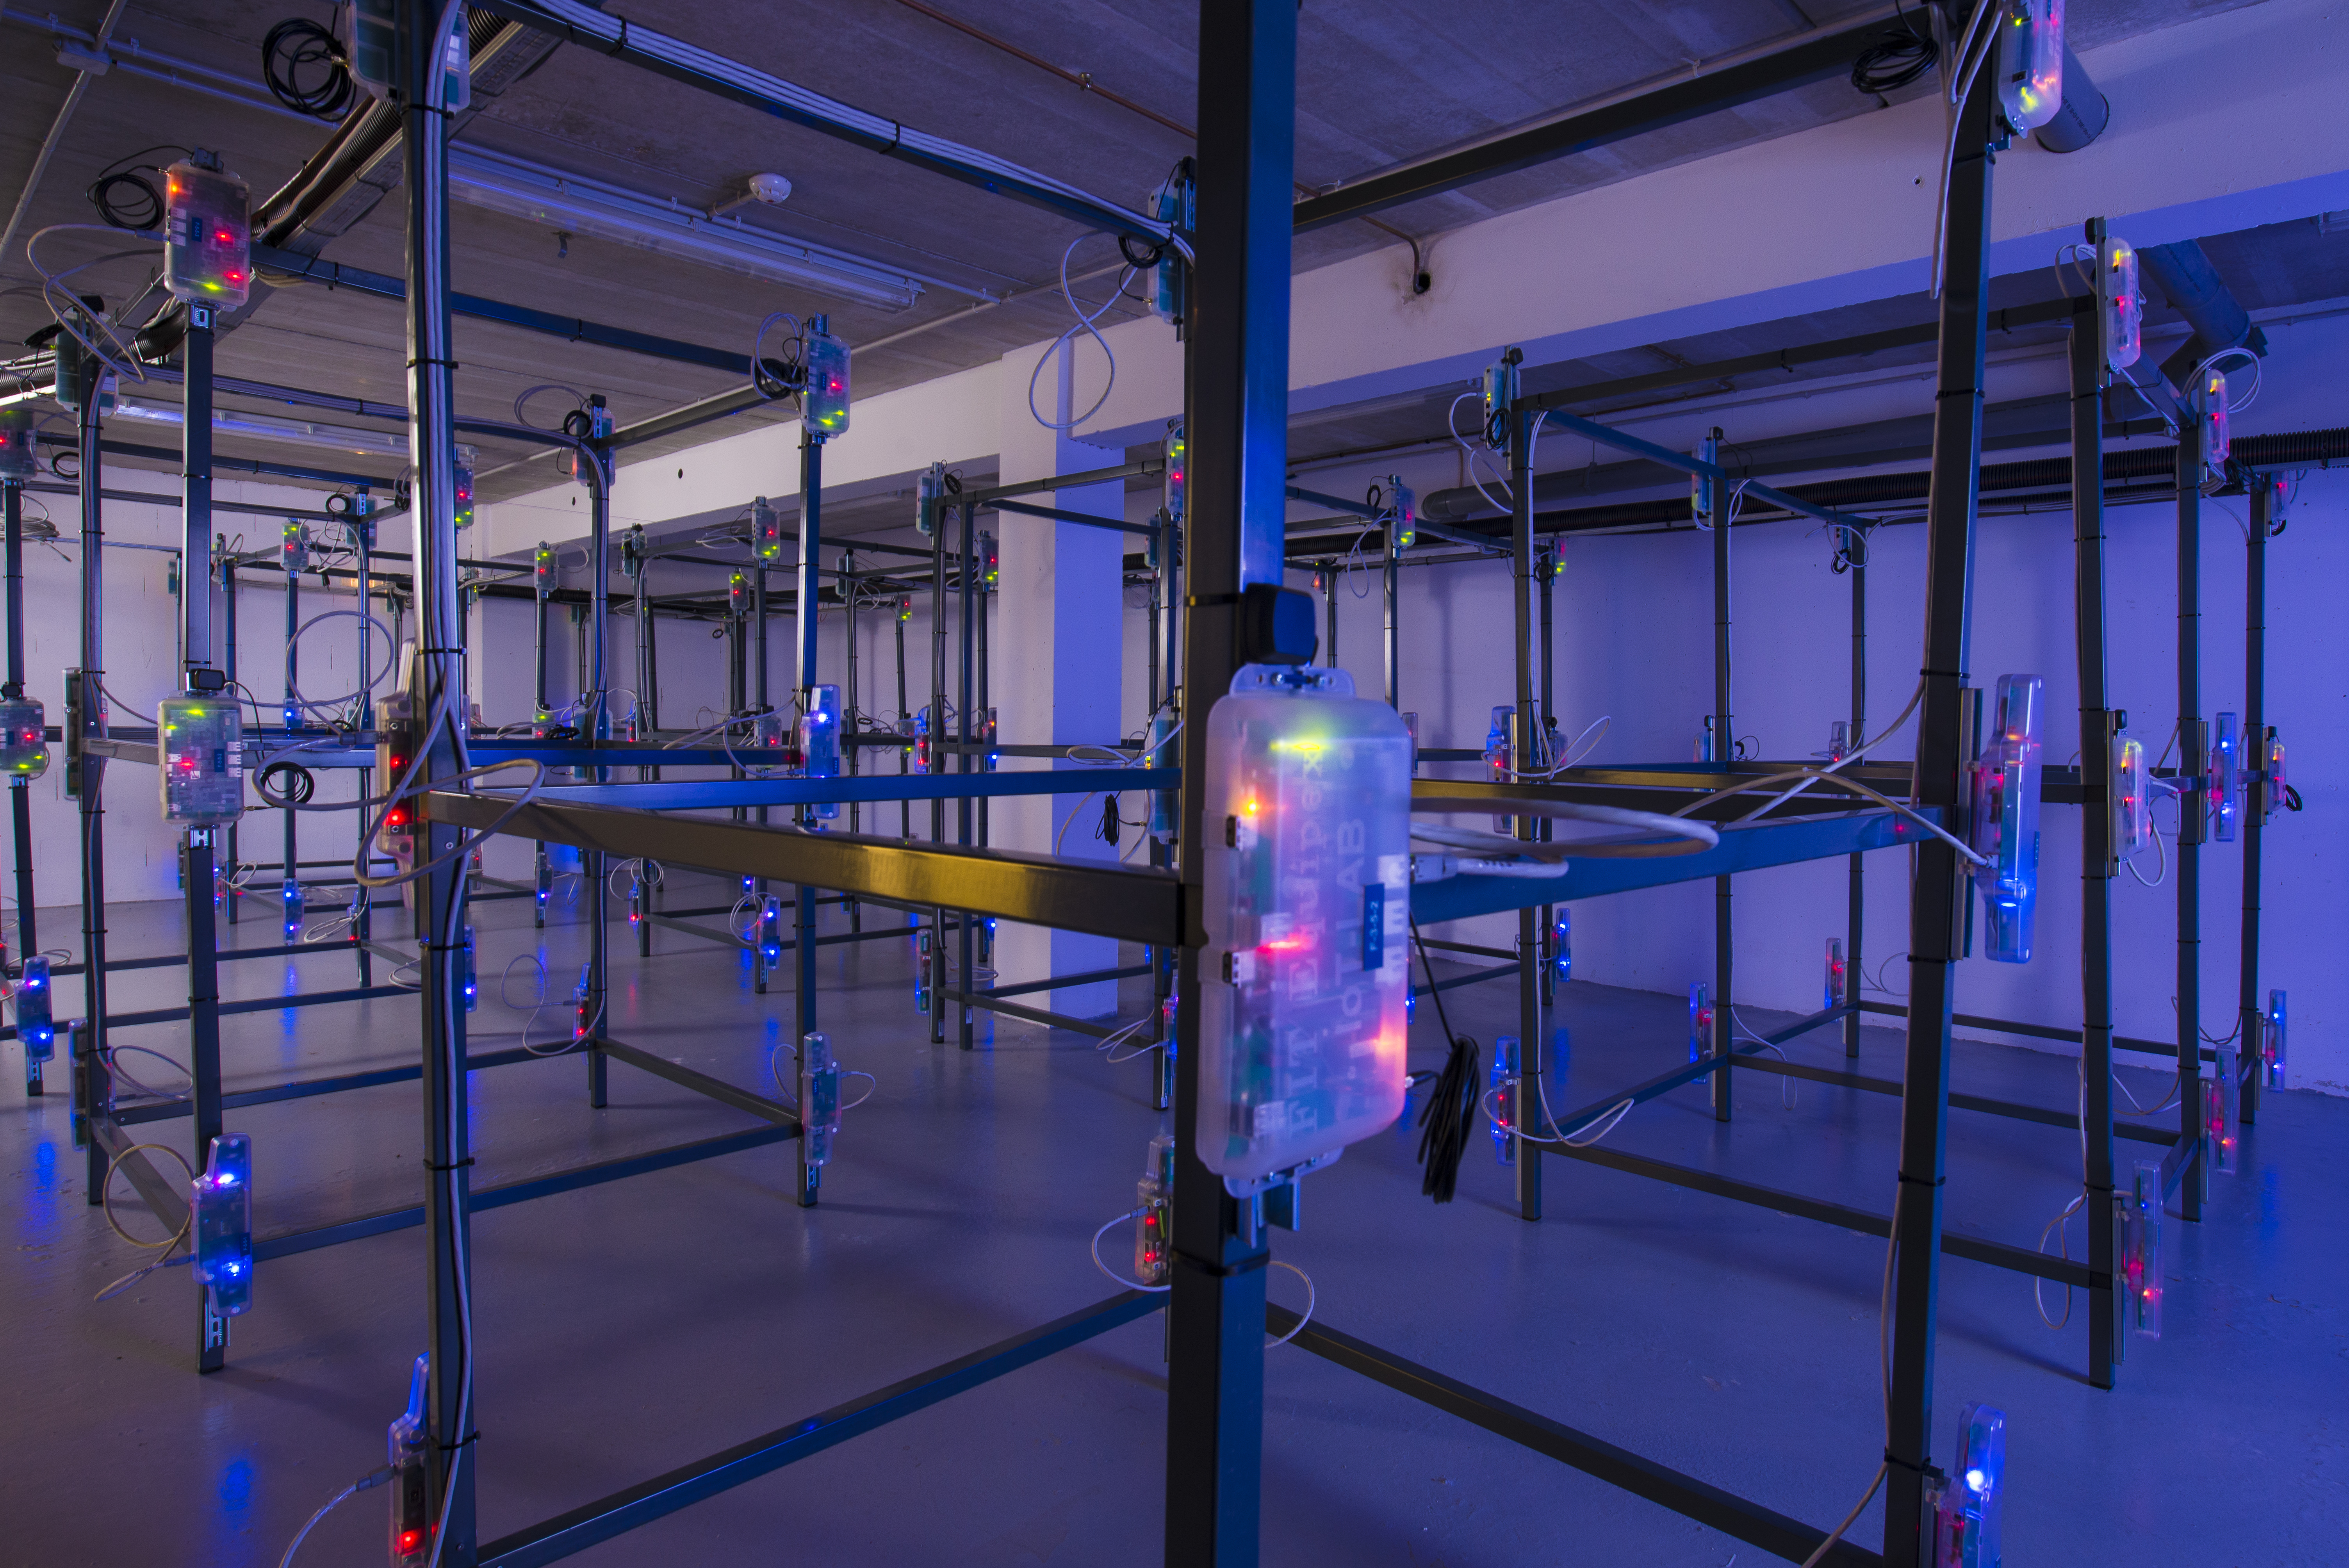
\includegraphics[width=\textwidth]{figures/iotlab.jpg}
%   \end{figure}

%   \pnote{
%     - Testbed où on teste les protocoles sur des plateformes matérielles diverses
%   }
%   \pnote{
%     - Déploiement simplifié permettant un passage à l'échelle plus simple.
%   }

% \end{frame}


% \begin{frame}{Smart Parking}
%   \begin{columns}
%       \begin{column}{0.48\textwidth}
%         \begin{figure}
%           % \centering
%           \includegraphics[width=0.8\textwidth]{figures/smart_parking.jpg}
%         \end{figure}
%       \end{column}
%       \begin{column}{0.48\textwidth}
%         \begin{block}{Avantages}
%           \begin{itemize}
%             \item Diminue le temps nécessaire pour trouver une place libre.
%           \end{itemize}
%         \end{block}
%         \begin{alertblock}{Projet Calipso}
%           \begin{itemize}
%             \item Déploiement à Barcelone
%           \end{itemize}
%         \end{alertblock}
%         \begin{figure}
%           \centering
%           \includegraphics[width=.7\textwidth]{figures/installation_smart_parking.jpg}
%         \end{figure}
%       \end{column}
%   \end{columns}
% \end{frame}


\begin{frame}{Contraintes et enjeux}
  \begin{block}{Contraintes}
    \begin{itemize}
      \item Faible cout $\implies$ économie d'énergie
      \item Capteurs hétérogènes et nombreux
      \item Longs déploiements (mois, années)
    \end{itemize}
  \end{block}
  \begin{alertblock}{Enjeux}
    \begin{itemize}
      \item Connecter ces objets à l'Internet
      \item Fournir du service à valeur ajouté
    \end{itemize}
  \end{alertblock}
\end{frame}

% \begin{frame}{Axes des contributions}
%   \begin{block}{Passerelle}
%     \begin{itemize}
%       \item Interface entre les réseaux contraints et classiques
%       \item Services pour le réseau de capteurs
%     \end{itemize}
%   \end{block}

%   \begin{alertblock}{Axes de contributions}
%     \begin{itemize}
%       \item Ajout de fonctionnalités transparentes pour le réseau de capteurs et les utilisateurs
%     \end{itemize}
%   \end{alertblock}

%   \pnote{
%     - Position clé à mi-chemin entre le monde contraint et le monde non contraint.
%     Plus facile d'y accéder qu'aux nœuds contraints.
%   }

%   \pnote{
%     Plus ressources car doit par exemple fournir une connectivité permanente par réseaux cellulaires, Ethernet.
%     Services supplémentaires: Pare-feux, sauvegarde des données collectées, mises à jour firmware, synchronisation d'horloge,
%     routeur de sortie, etc.
%   }
%   \pnote{
%     - Comment ajouter des fonctionnalités utiles et transparentes pour les noeuds ?
%   }

% \end{frame}
